\section{Introduction}\label{sec:introduction}
This chapter shows screenshots of the system interface, connections of the hardware equipment and other details the programming environment that was used to develop the system.


\section{Implementing the system}

\subsection{Programming Tools}
The system was implemented using the following programming tools:
\begin{itemize}
    \item \textbf{Android Studio}: This is the official IDE for Android development. It was used in the development of the mobile application.
    \item \textbf{Arduino IDE}: This is the official IDE for Arduino development. It was used in the development of the microcontroller code.
    \item \textbf{Digital Ocean}: This is a cloud hosting service. It was used to host the remote server.
    \item \textbf{Flutter}: This is a cross-platform UI toolkit developed by Google. It is used to develop the mobile application.
    \item \textbf{Firebase}: This is a mobile and web application development platform developed by Google. It is used to handle user authentication.
    \item \textbf{Silicon Pay}: This is the payment gateway the researchers opted for due to its support for all local payment platforms
    \item \textbf{ESP32 Microcontroller}: This is a microcontroller developed by Espressif Systems. It is used to receive data from the mobile application and send it to the remote server.
    \item \textbf{Servo Motor}: This consists of a DC motor, gearbox, and a control circuit. It has a simple lever that can be attached to it and used to demonstrate the opening and closing of the gate upon verification of payment.
    \item \textbf{FTDI connector}: This is a USB to serial adapter that is used to program the ESP32 microcontroller.
\end{itemize}

\clearpage

\subsection{Embedded Systems Equipment}
The following equipment was used in the development of the system:
\begin{figure}[h]%
    \centering
    \subfloat[\centering]{{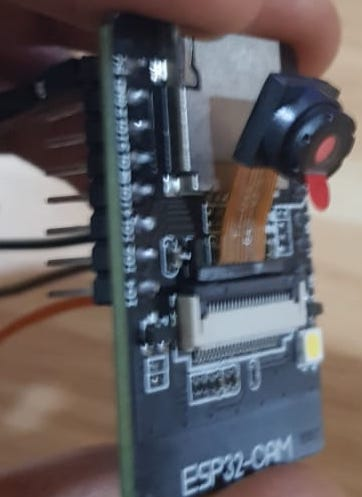
\includegraphics[scale=0.32]{images/esp1} }}%
    \qquad
    \subfloat[\centering]{{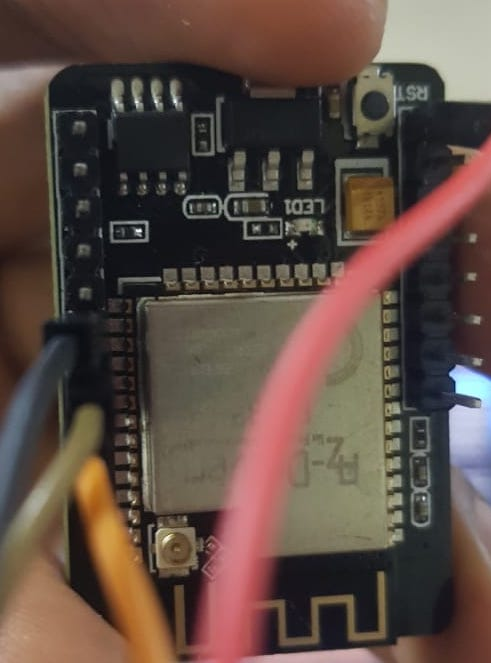
\includegraphics[scale=0.24]{images/esp2} }}%
    \caption{ESP32 microntroller used to scan the user QR codes}%
    \label{fig:equip}%
\end{figure}
\begin{figure}[h]
    \centering
    \subfloat[\centering]{{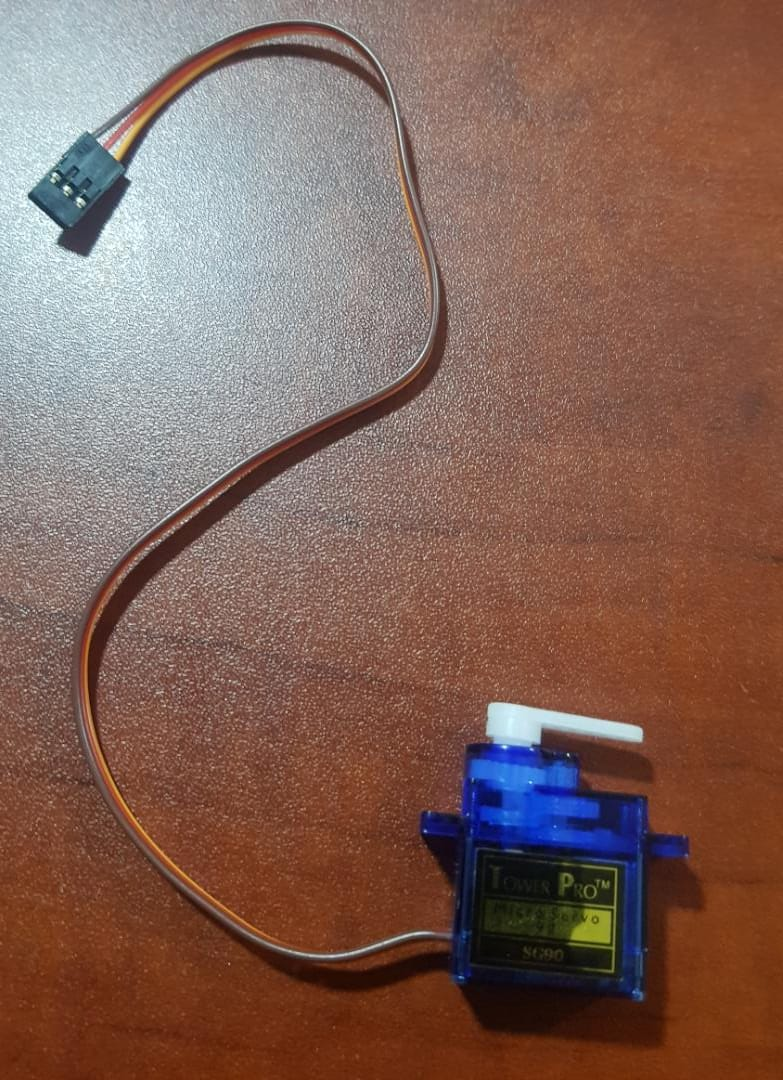
\includegraphics[scale=0.12]{images/servo} }}%
    \qquad
    \subfloat[\centering]{{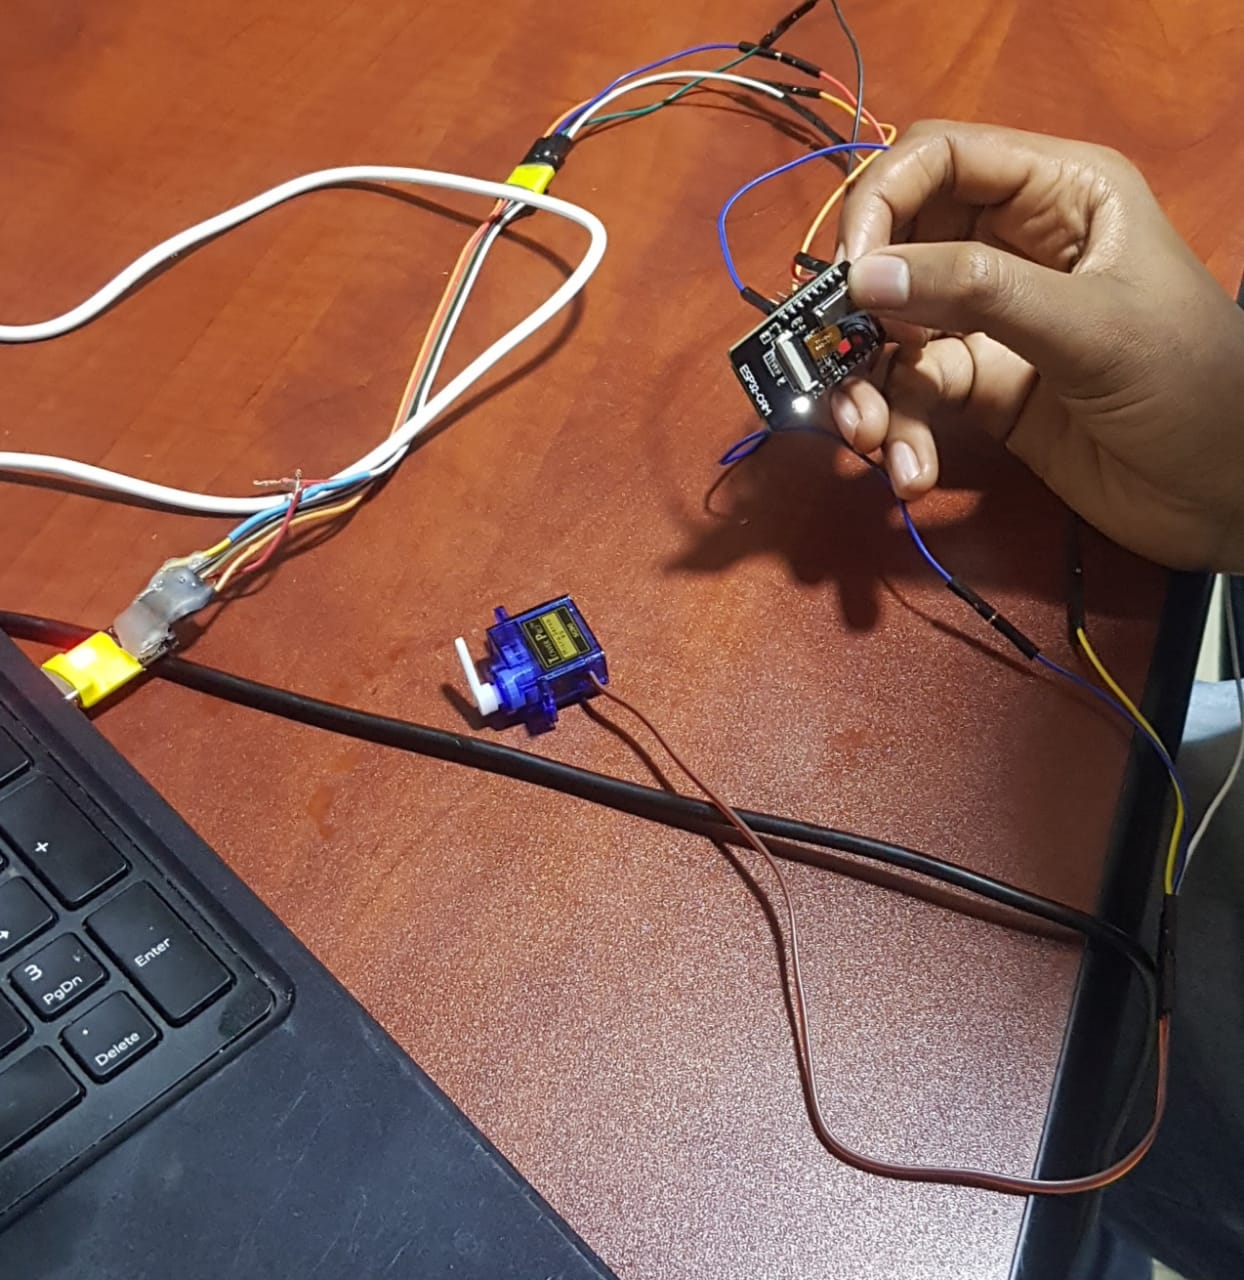
\includegraphics[scale=0.1]{images/full-connection} }}%
    \caption{Left is a servo motor used to demonstrate closing and opening logic and Right is the complete connection of the equipment }%
    \label{fig:equip}%
\end{figure}
\clearpage

\subsection{Screenshots of the mobile application in order of use}
\begin{figure}[h]%
    \centering
    \subfloat[\centering]{{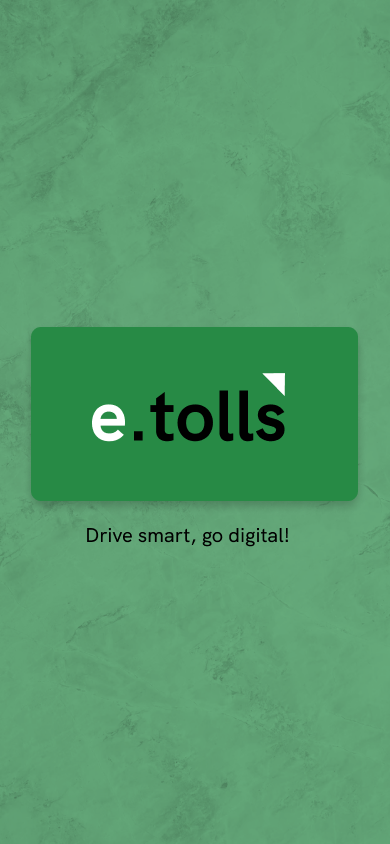
\includegraphics[scale=0.17]{images/Splashscreen} }}%
    \subfloat[\centering]{{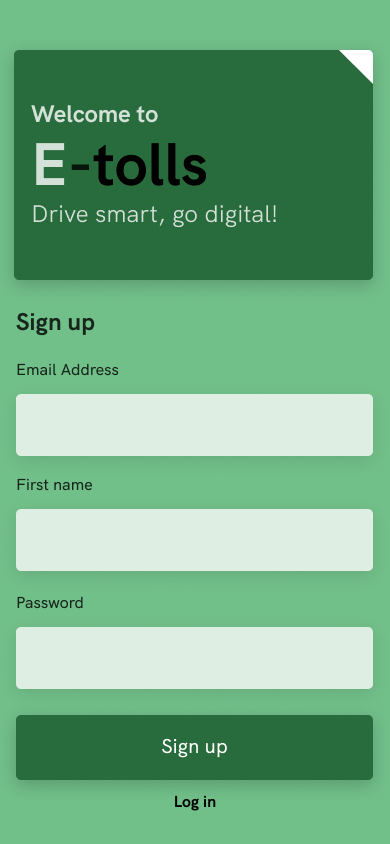
\includegraphics[scale=0.17]{images/Signup} }}  \subfloat[\centering]{{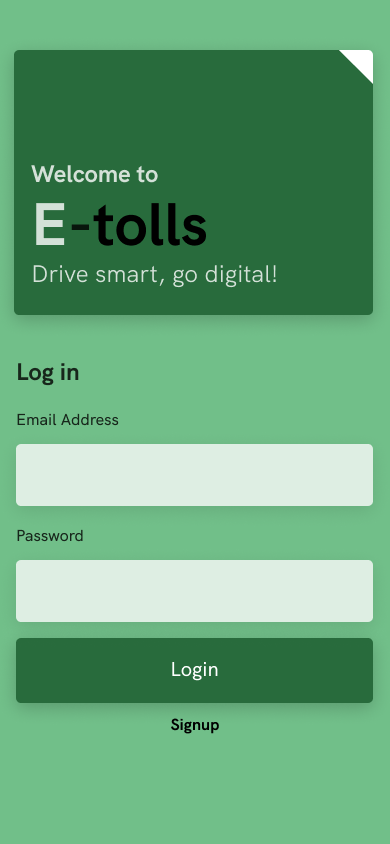
\includegraphics[scale=0.17]{images/Log in} }}%
    \caption{Login and Sign Up Screens of the mobile application}%
    \label{fig:example}%
\end{figure}
\begin{figure}[h]%
    \centering
    \subfloat[\centering]{{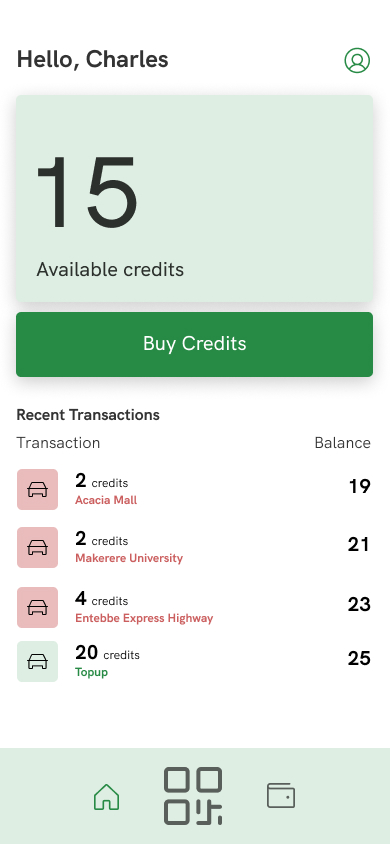
\includegraphics[scale=0.17]{images/Home} }}%
    \subfloat[\centering]{{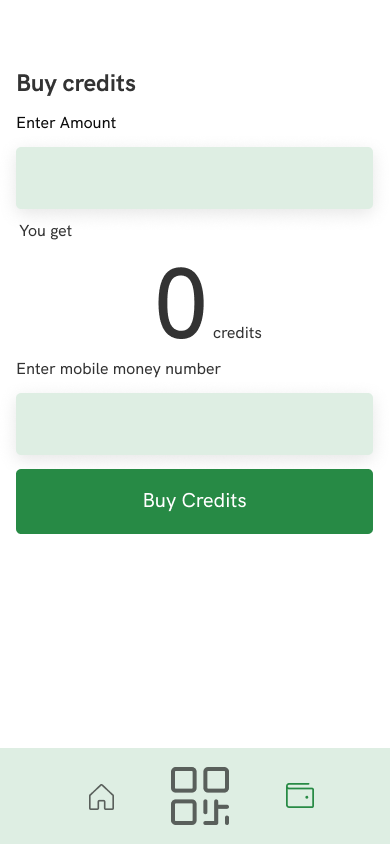
\includegraphics[scale=0.17]{images/Payments} }}%
    \subfloat[\centering]{{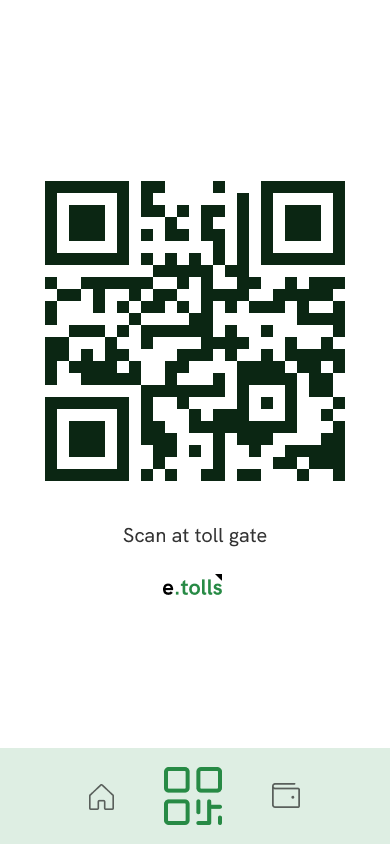
\includegraphics[scale=0.17]{images/QRCode} }}%
    \caption{Home & Payment Screens of the mobile application}%
    \label{fig:example1}%
\end{figure}

\clearpage
\subsection{Silicon Pay Administrator dashboard}
THe payment gateway Silicon Pay also provides a web based dashboard which one can use to monitor transactions made through the system. The dashboard is shown below:
\begin{figure}[h]
    \begin{center}
        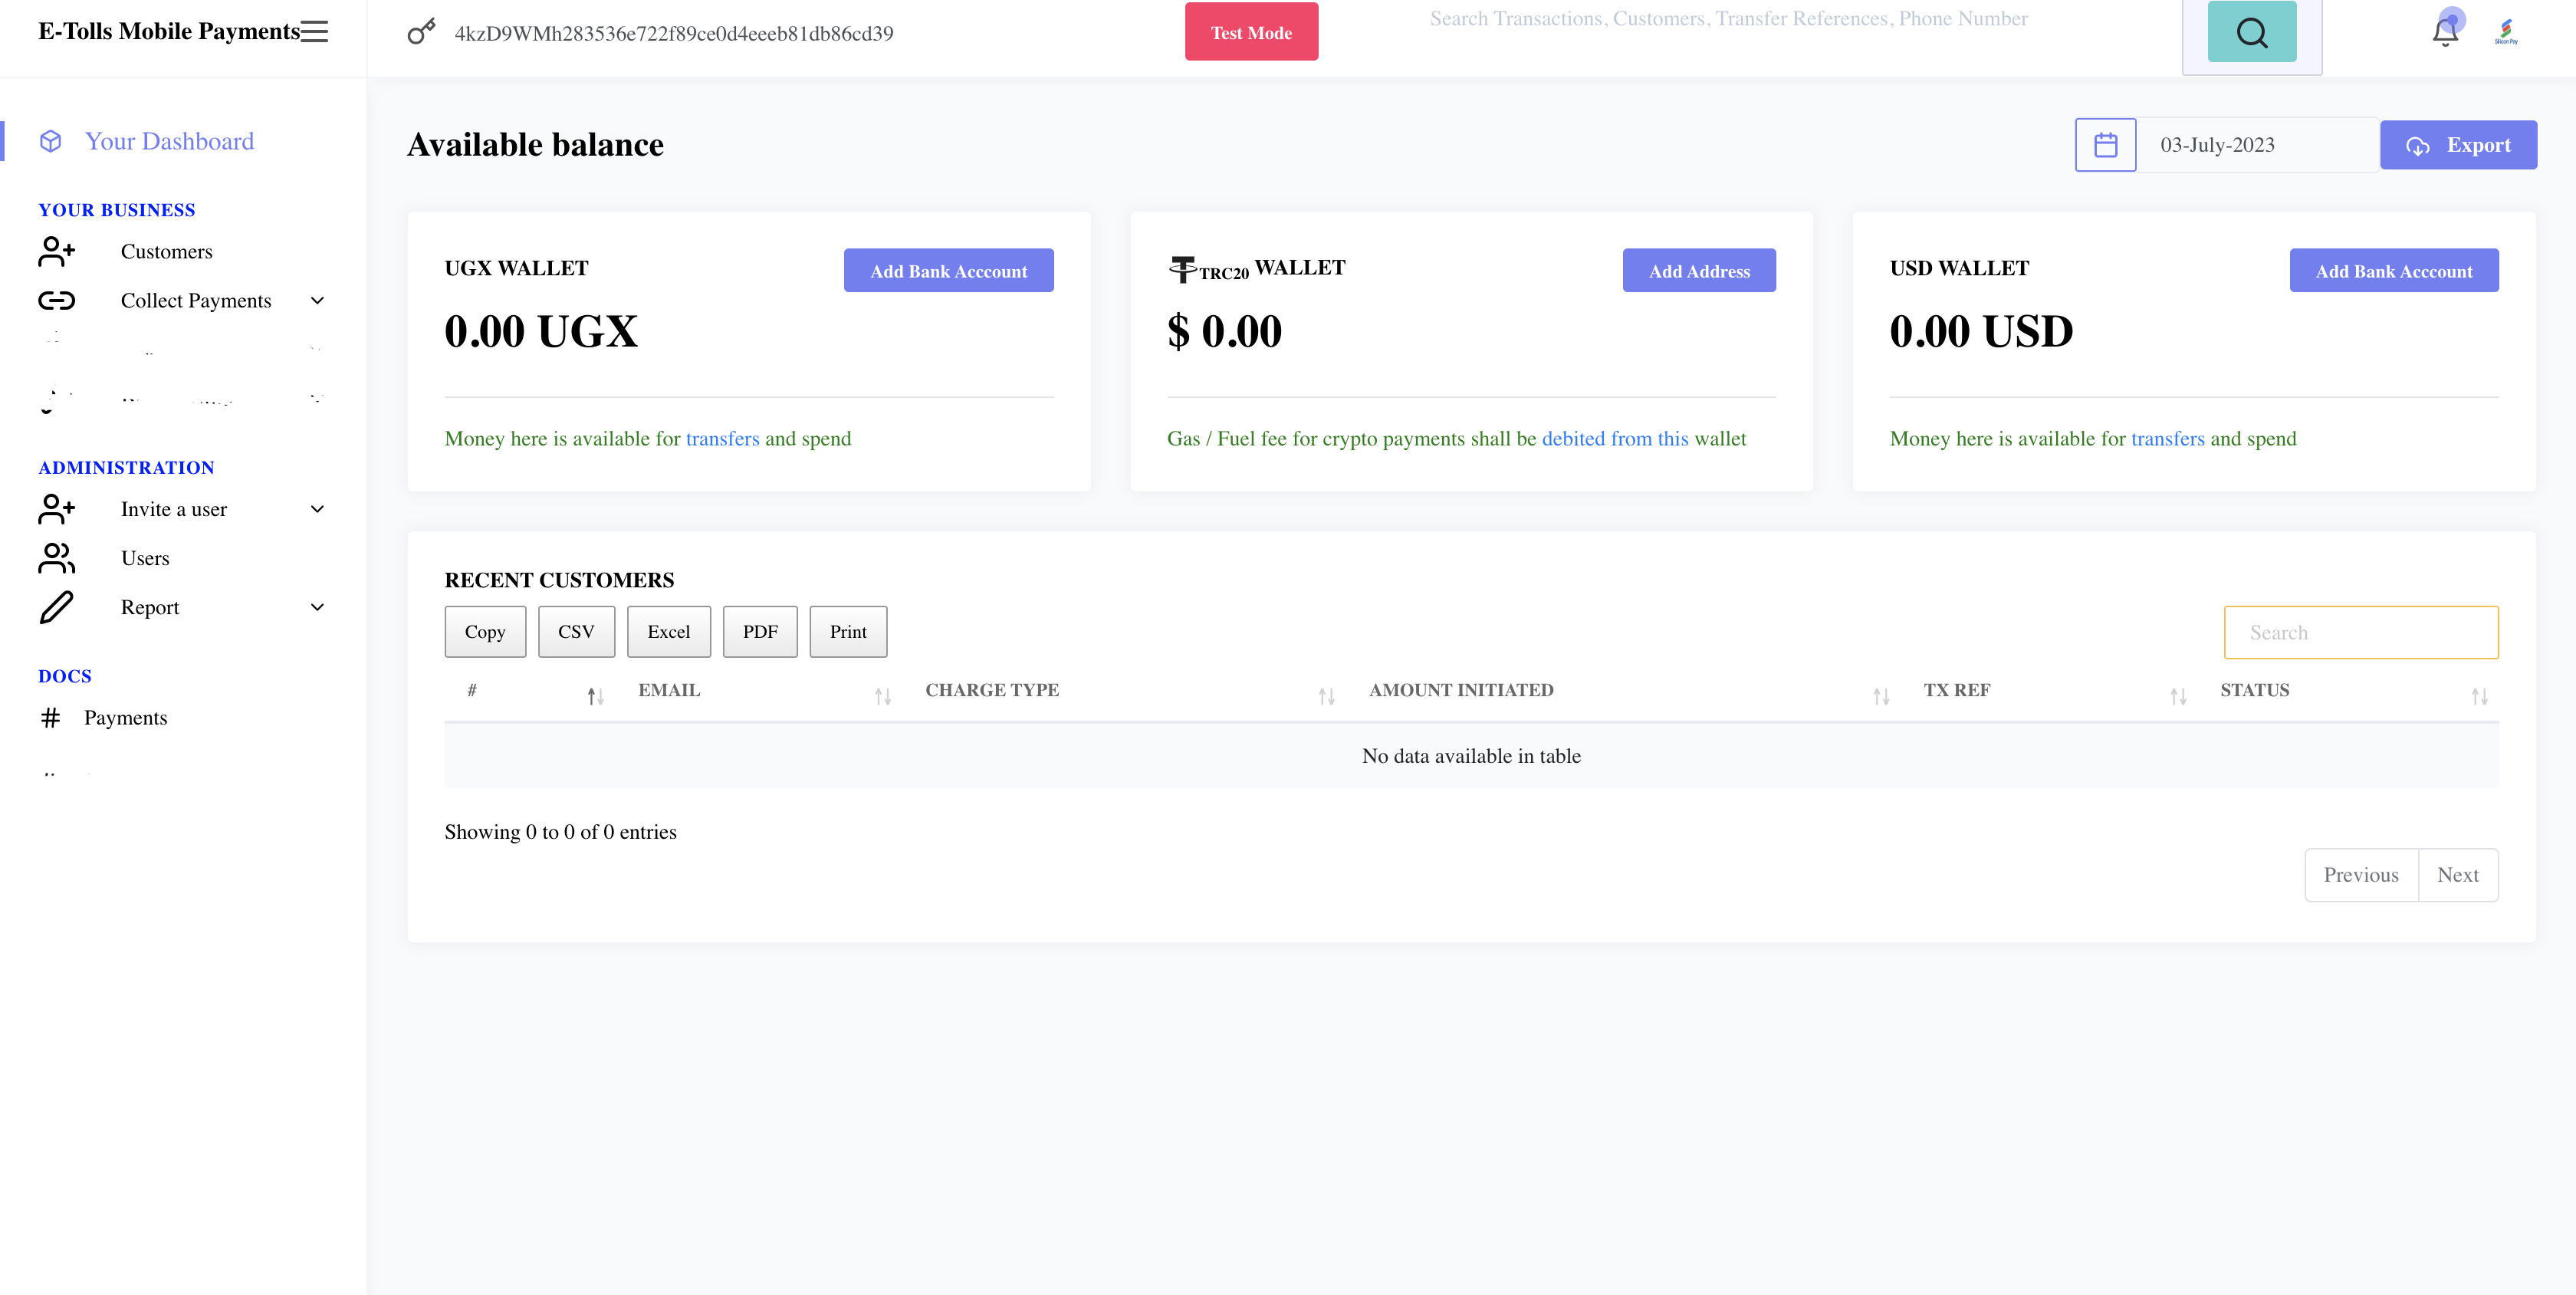
\includegraphics[scale = 0.1]{images/dashboard_1}
        \caption{Web based admin dashboard to view all transactions}
    \end{center}
\end{figure}


\begin{figure}[h]
    \begin{center}
        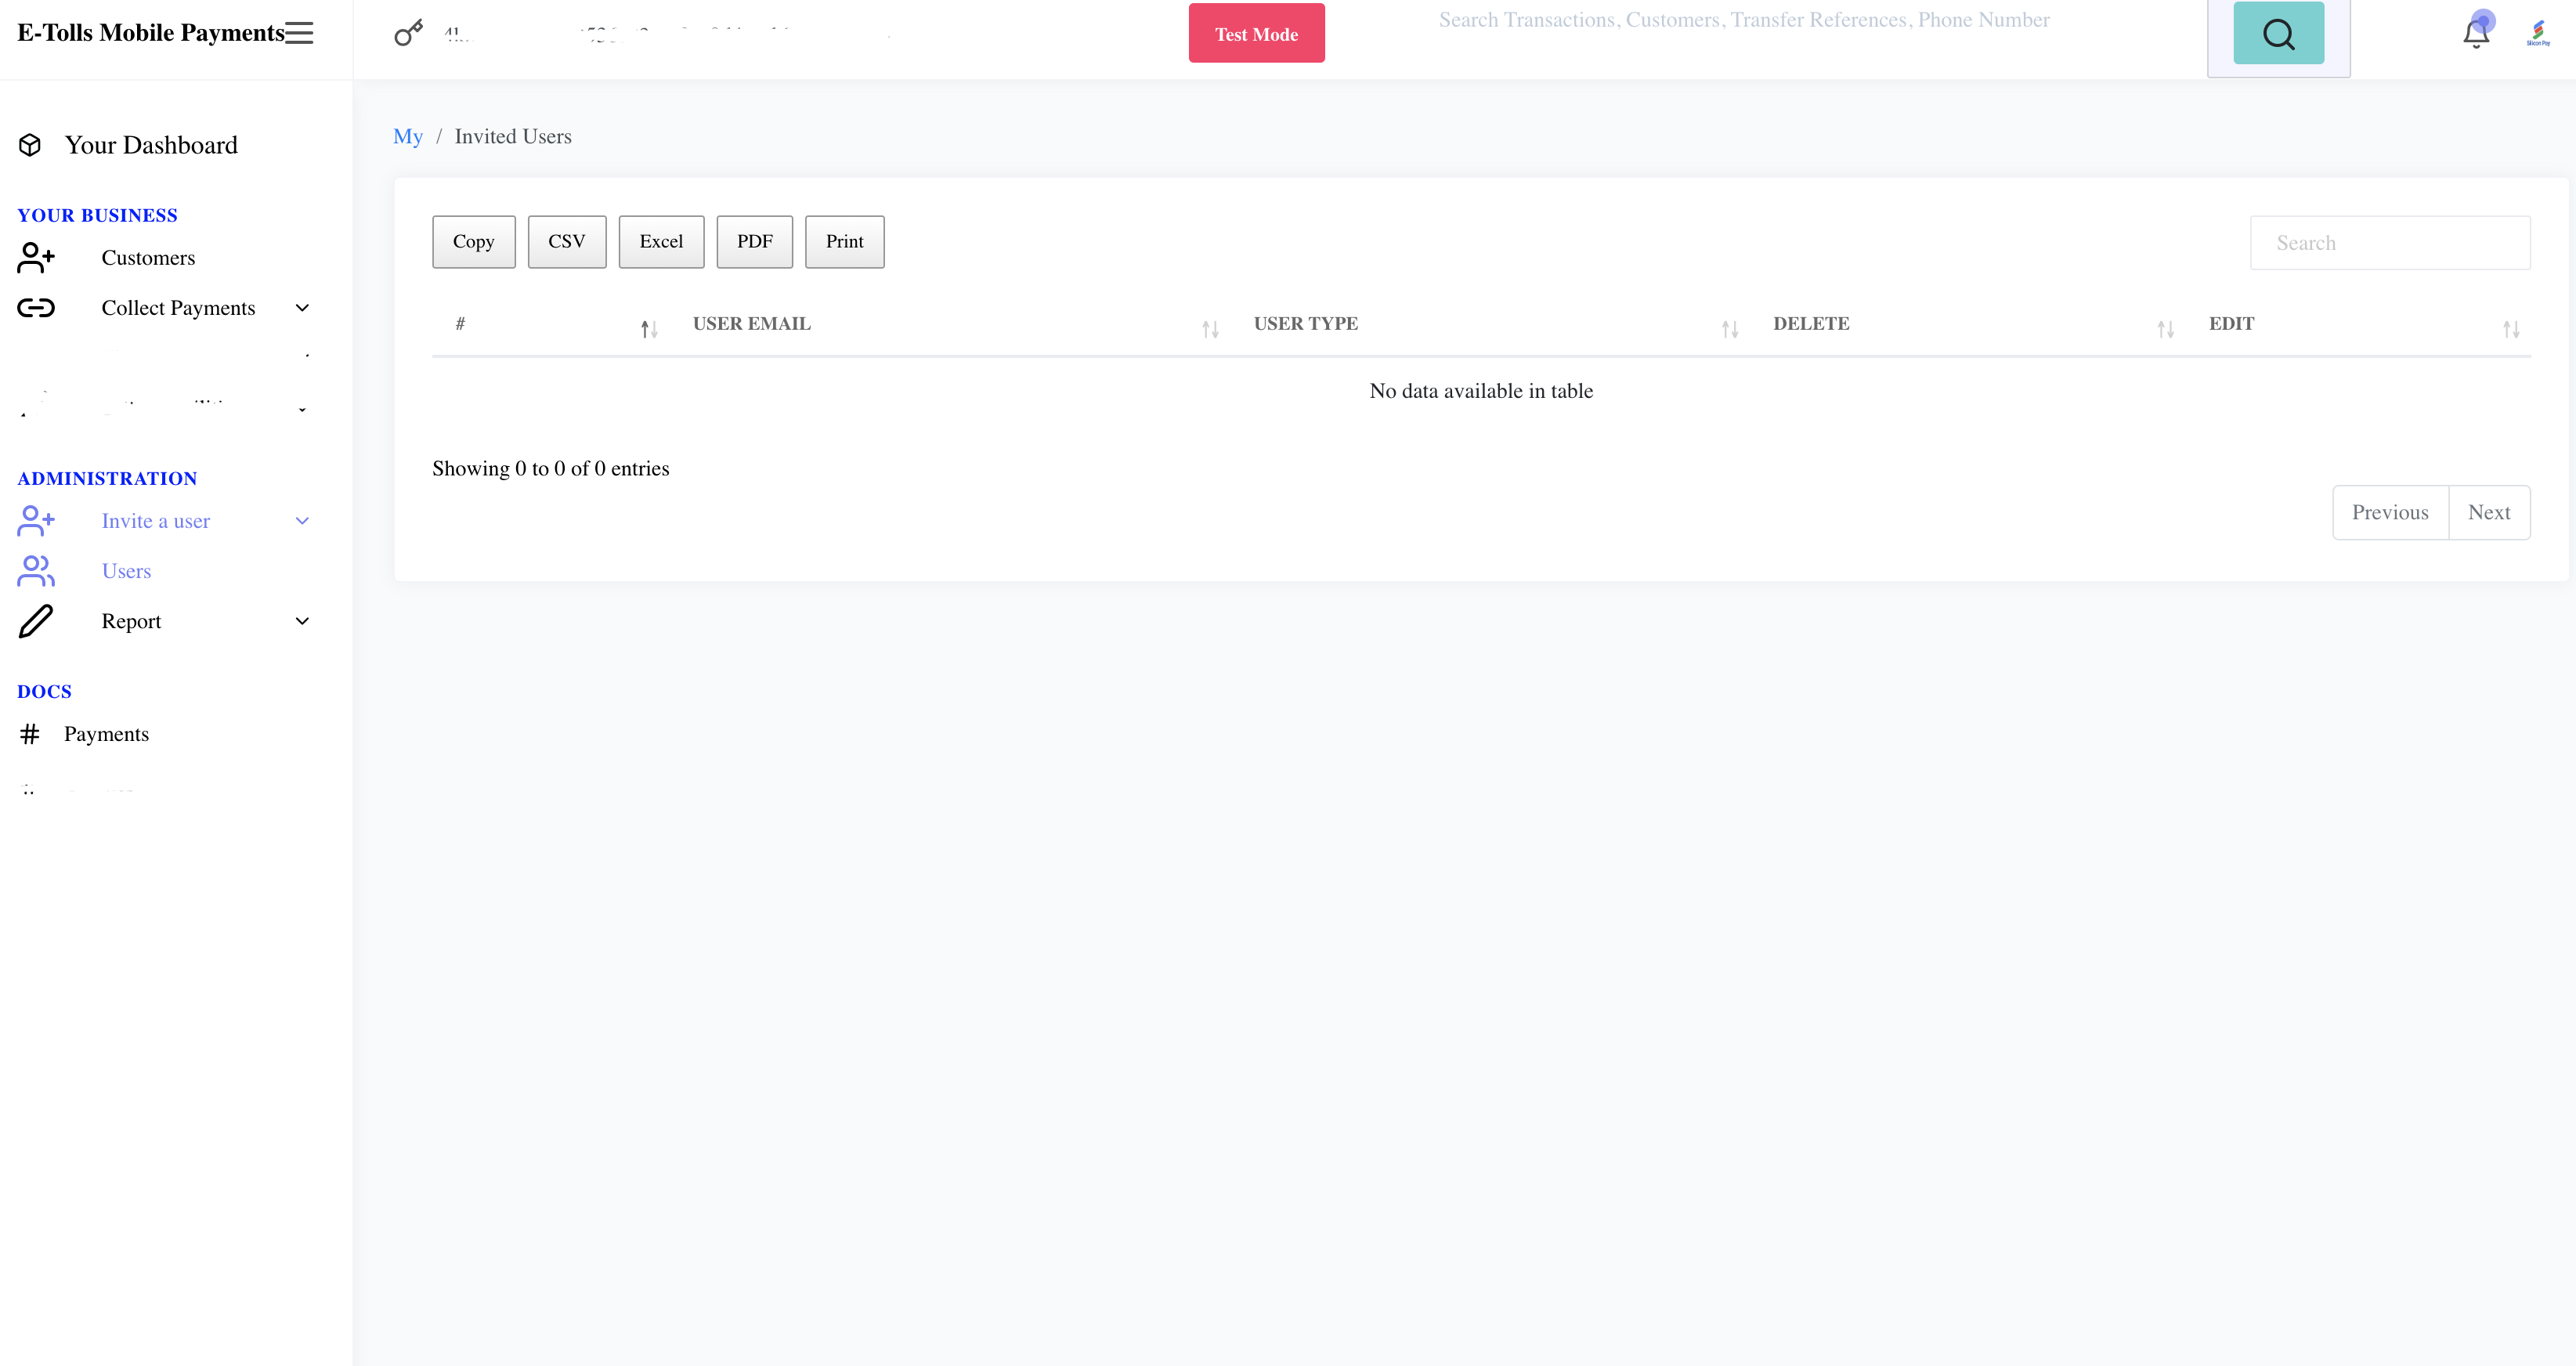
\includegraphics[scale = 0.1]{images/dashboard_2}
        \caption{Table to hold summary of customers data that can be exported as CSV/PDF}
    \end{center}
\end{figure}

\begin{figure}[h]
    \begin{center}
        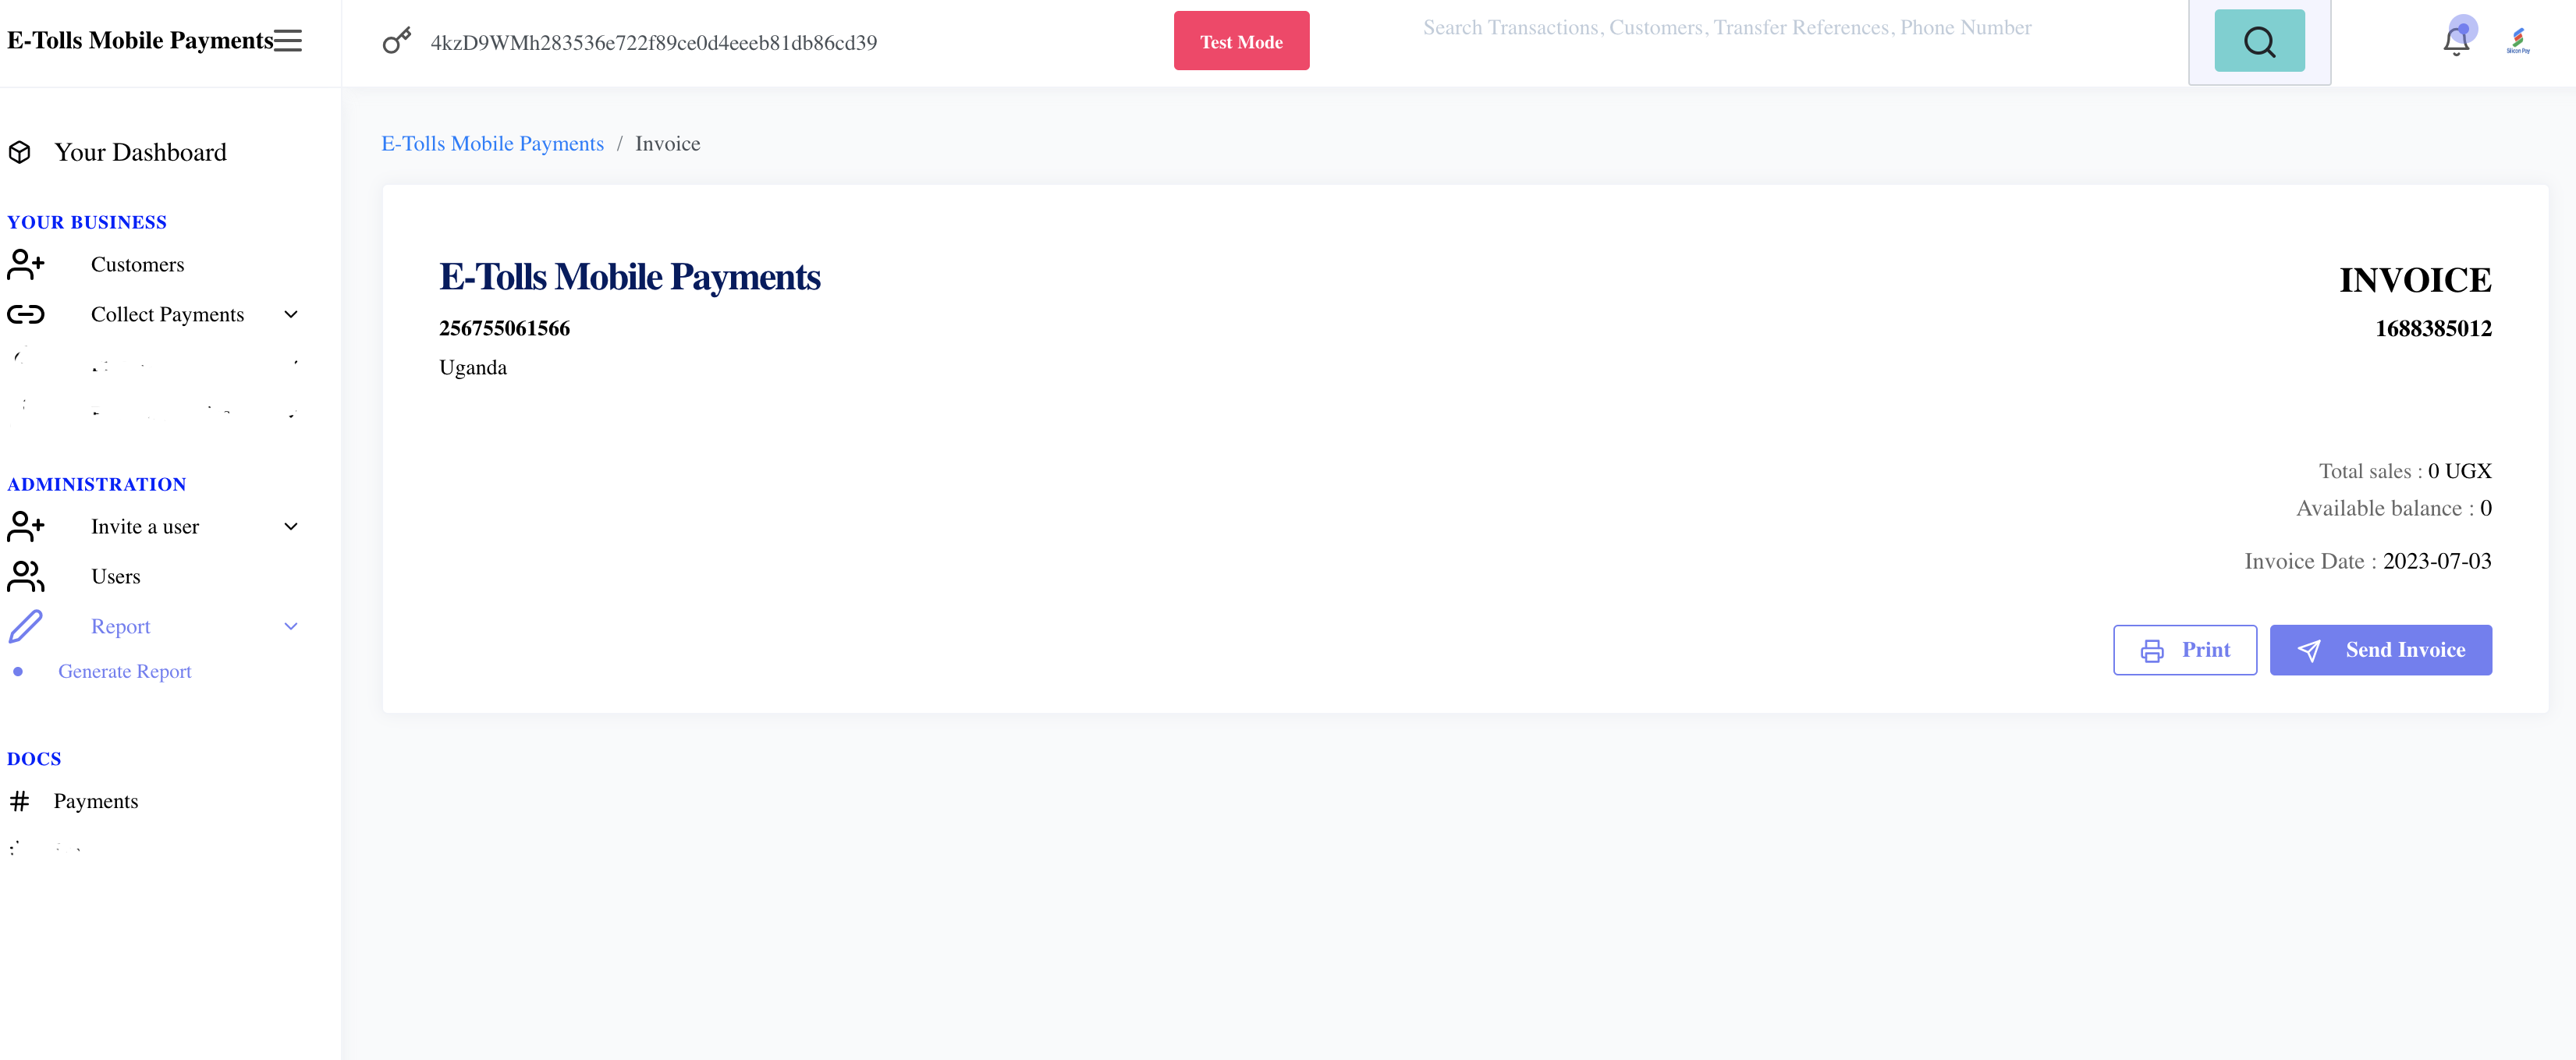
\includegraphics[scale = 0.1]{images/dashboard_3}
        \caption{ General Report of transactions made in a given period of time}
    \end{center}
\end{figure}

